\subsection{Design of the Data Management}
\label{subsec:designdatamanagement}

A lot of data is involved in the application. This ranges from user information to recipe information and preferences. This provides a challenge on how to manage data, both for the client itself but also in combination with the backend. Android does support that one can extend the \texttt{Application} class, which means that any information stored there, is available in all instances of \texttt{Activity}. But this solution comes with problems, see \citep{application_storage}. Other solutions are however possible, and the following is what was done in this project in order to handle different kinds of data.

\subsubsection{Bundles and Intents}
\label{subsubsec:bundles_and_intents}

As can be seen in \ref{sec:patterns}, instances of \texttt{Activity} has their own lifecycles. They are created and they run. At some point they are stopped and finally destroyed. Since an \texttt{Activity} only represents one screen, this chain of events occurs often. The problematique, seen from a data perspective is that everything that was created, calculated or altered in that Activity dies with it.
A concrete example could be upon opening a recipe from somewhere within the application. This would create an instance of a \texttt{RecipeActivity}. The \texttt{Activity} from which it was launched is then either destroyed or paused, depending on whether it should be possible to return to it later. The \texttt{RecipeActivity} needs information on the recipe to show, but the two instances of \texttt{Activity} can not communicate as they please.

For a case like this, the solution is to manage the information through \texttt{Intent} or the more specific \texttt{Bundle}. These two features are standard Android classes that allows the creation of a new \texttt{Activity} to be associated with a \texttt{Bundle} and/or \texttt{Intent} containing information\cite{intent}\cite{bundle}. Both classes can hold a variable amount of pre-defined data types such as \texttt{char}, \texttt{string}, \texttt{double} and many more.

To return to the example, that does not entirely solve the problem. The pre-defined data types means that a recipe can not be passed through an \texttt{Intent} or \texttt{Bundle}. This is solved in the application by converting the recipe to JSON, and then passing it as a simple string containing the JSON.

\subsubsection{SharedPreferences}
\label{subsubsec:sharedpreferences}

Another potential issue by using \texttt{Bundle} or \texttt{Intent} is that this only works well when the data is used immediately after, in the \texttt{Activity}  that was just created. In some cases, data is created or available ahead of time. In these cases it is a waste to keep passing data back and fourth through several \texttt{Activity} instances until one instance finally needs the data. This can be solved through a more persistent storage solution called \texttt{SharedPreferences}. This is another Android class which enables the creation, manipulation and deletion of a file which is only accessible from the application that created it\cite{sharedpreferences}. This does however not mean that the data is completely secured, see \citep{sharedpreferences_security}.

To exemplify where this is useful, consider the process of logging in. The user inputs e-mail address and password. The server verifies this, and returns the ID of the user. This ID is used several times in the application, examples being fetching the list of favorite recipes, preferences, settings and user information. It would be inconvenient to pass it continuously between different parts of the application. By using \texttt{SharedPreferences}, they can be fetched whenever they are needed.

Furthermore, this is how the application checks whether a user should login when opening the application. If a file exists due to stored \texttt{SharedPreferences}, then there is no reason to login - the required information is already available. Otherwise the user will have to login which creates a new file with the relevant user data. The process of checking this situation can be seen in \ref{lst:login_check}. The listing shows the attempt to locate a file, matching the name of the value stored in \texttt{R.string.app\_name}. If the file is found, it should contain some information about the user - an example being \texttt{alias} as in the listing, but other checks should work as well. If the instance of \texttt{SharedPreferences} contains the \texttt{alias} variable, the \texttt{LoginActivity} is ended immediately, skipping to the next screen, the \texttt{PagerActivity}.

\subsubsection{Server}
\label{subsubsec:server}
The server presents the biggest challenge in terms of data management. The structure used to overcome this challenge can be seen in \ref{fig:application_dataflow}. The application has to match models that are recognized by the server, in order for the communication to make sense. The responsibility of using these models are placed on the \texttt{Activity}.

The \texttt{ServiceHelper} provides an interface to the server. It consists of methods that matches the functionality provided by the server. This is where the facade pattern mentioned in \ref{sec:patterns} becomes practical. For the programmer working on the \texttt{Activity} level, there is no need for knowledge about the server. The \texttt{ServiceHelper} works as a facade, only requiring the \texttt{Activity} programmer to choose the appropriate method and providing any parameters needed. This could for example be one of the models.

\begin{figure}[H]
	\centering
	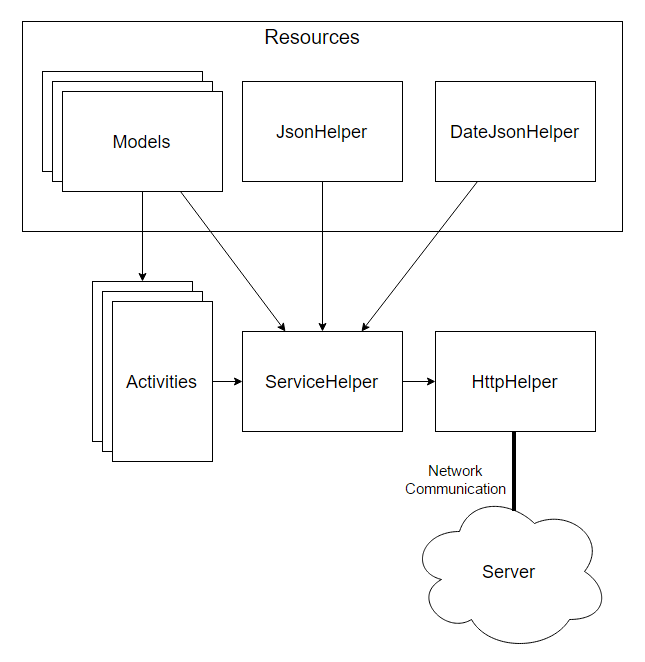
\includegraphics[width=\textwidth]{Pictures/application_dataflow.png}
	\caption{Processing data for server communication}
	\label{fig:application_dataflow}
\end{figure}

The \texttt{ServiceHelper} puts together the necessary steps to actually communicate with the server. This involves creating a request the server can recognize, converting it to JSON, and sending it to the correct URL. The first two tasks are however generic and can be formulated outside the context of a specific server request. As such the \texttt{ServiceHelper} has the information on where a request should be sent URL-wise, but uses further helper classes for providing JSON serialization/deserialization (\texttt{JSONHelper})and creating HTTP requests(\texttt{HTTPHelper}).

The \texttt{HttpHelper} puts together the HTTP request (address, content, request type is passed from the \texttt{ServiceHelper}) and sends it to the server. If all goes well, the server sends back a response. This response is then treated with the reverse process. It is deserialized from JSON into a usable format (simple types or one of the models), and returned to the \texttt{Activity} via the \texttt{ServiceHelper}.

The total running time of a process such as this can vary depending on the computations required from the server request and the network delay. Furthermore there is always the risk of dropping out on a mobile device, failing the network connection. For this reason, networking is done on a separate thread. This ensures that the UI will not hang, with the worst case scenario of Android telling the user the application is not responding. In fact, any attempt to do networking on an applications main thread will cause Android to throw an exception by default (for Android 3.0 and above)\cite{networking_mainthread}.

In practice the multi-threading is done using Android's \texttt{AsyncTask} class. This enables the use of asynchronous threading. In effect, the thread that creates an \texttt{AsyncTask} can continue unhindered, collecting the result of the task when convenient\cite{asynctask}.

A last thing to note according to \ref{fig:application_dataflow} is the \texttt{DateJsonHelper}. This class is a workaround to deal with inconsistent data types. Both the Java (Frontend) and C\# language (Backend) provides data types for dealing with time and date. Given the availability of this, it would make little sense to implement this functionality from the ground up. The two implementations are however different from each other in that Java is zero-based while C\# is not. An example of where this goes wrong is simply by sending a month from the server to the application. Sending January (1) would be parsed by Java as Feburary, while December would be invalid altogether, as 12 is out of range for Java.
Rather than manually implement all the functionality needed for date and time, the \texttt{DateJsonHelper} was created to ensure that the formats become compatible with the receiving end, whether it is on deserialization of JSON for the application or serialization for the server.